\documentclass{standalone}
\usepackage{tikz}
\usepackage{ctex,siunitx}
\usepackage{tkz-euclide}
\usepackage{amsmath}
\usetikzlibrary{patterns, calc}
\usetikzlibrary {decorations.pathmorphing, decorations.pathreplacing, decorations.shapes,}
\begin{document}
\small
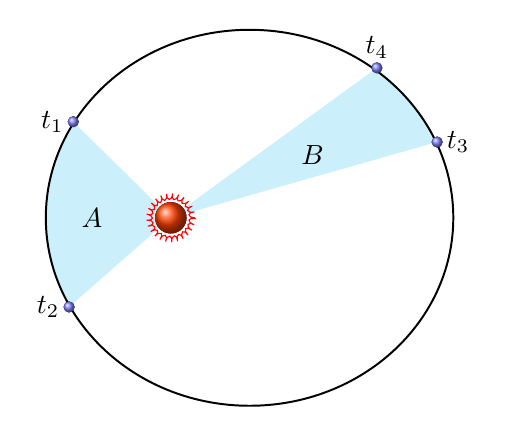
\begin{tikzpicture}[>=stealth,scale=1]
  \begin{scope}
  \path [clip](0,0)ellipse(2.6 and 2.4);
  \fill[cyan!20](-2.239,1.22)--(-1,0)--(-2.292,-1.133)to[bend left]cycle;
  \fill[cyan!20](1.617,1.904)--(-1,0)--(2.382,0.962)to[bend right]cycle;
  % \fill[cyan!20](1.434,-2.002)--(-1,0)--(0,-2.4)to[bend right]cycle;
  \fill[ball color=orange!50!red](-1,0)circle(0.2);
  \draw[red,decoration={bumps,segment length=1.5mm,amplitude=0.7mm},decorate] (-1,0) circle (0.3);
  \draw[line width =0.5mm](0,0)ellipse(2.6 and 2.4);
  \end{scope}
  \foreach \x/\y/\lc [count =\i] in {-2.239/1.22/left,-2.292/-1.133/left,2.382/0.962/right,1.617/1.904/above}
  {
    \fill[ball color=blue!50] (\x,\y)circle(2pt)node[\lc]{$t_\i$};
  }
  \node at (-2.0,0.0) {$A$};
  \node at (0.8,0.8) {$B$};
\end{tikzpicture}
\end{document}